
\documentclass[ms.tex]{subfiles}

\begin{document}

\section{Observational Diagnostics}
\label{sec:diagnostics}

\begin{itemize}

	\item If the SN Ia rate indeed depends on metallicity with a
	$\sim Z^{-\gamma}$ dependence where~$\gamma \approx -0.5$, then in principle
	this should impact the scaling of the specific SN Ia rate with stellar mass
	at different redshifts due to the redshift-evolution of the MZR.
	To investigate this, we take the same~$z = 0$ stellar masses spanning
	$10^{7.2} - 10^{12}~\msun$ and determine their corresponding stellar masses
	at redshifts of~$z = 0.5$ and 1 by integrating the SFH up to the
	appropriate lookback time (we assume the cosmological parameters measured
	from the cosmic microwave background in~\citealt{Planck2014} and compute
	the lookback times using~\textsc{astropy}).
	We then evaluate the~\citet{Zahid2014} MZR at the implied stellar mass for
	the appropriate redshift and evaluate the specific SN Ia rate according to
	equation~\refp{eq:specia} with the lower bound of each integral replaced
	with the lookback time to the given redshift, applying a~$Z^{-0.5}$
	correction to compute the metallicity-dependent rates.
	To compare to a case where~$\gamma = 0$, we omit the~$Z^{-0.5}$ correction
	and instead apply an additional~$(M_\star / 10^{10}~M_\odot)^{-0.15}$
	prefactor to account for the shallower scaling predicted when~$\gamma = 0$
	as opposed to~$\gamma = -0.5$.
	This prefactor brings the~$\gamma = 0$ case into better agreement with the
	$\gamma = -0.5$ case at~$z = 0$ and is intended to encapsulate the
	otherwise unknown processes which amplify the SN Ia rate at low stellar
	masses if it is instead not due to metallicity effects.
	We nonetheless caution that this is a purely~\textit{a posteriori}
	correction not based on physical arguments so that we can make an
	``apples to apples'' comparison between two models which agree with
	an~$M_\star^{-0.3}$ scaling at~$z = 0$ as measured by~\citet{Gandhi2022}.

	\item We plot the resulting specific SN Ia rates as a function of stellar
	mass at~$z = 0$, 0.5, and 1 in the left panel of Fig.~\ref{fig:specia_zdep}.
	We clarify that the stellar masses correspond to the appropriate redshift.
	That is, the rates at, e.g.,~$z = 1$ are normalized to the rate determined
	for a galaxy with a stellar mass of~$M_\star = 10^{10}~M_\odot$ at $z = 1$
	but would be more massive on average at the present day.
	In either the~$\gamma = 0$ or~$\gamma = -0.5$ case, the specific SN Ia
	rates decrease at low stellar masses with increasing redshift.
	If~$\gamma = -0.5$, these calculations suggest that it should decrease by a
	factor of~$\sim$2 between~$z = 0$ and 1 at~$M_\star \approx 10^{7.2}~\msun$,
	the lowest stellar mass for which we have made predictions at all 3
	redshifts.
	If instead~$\gamma = 0$, the rate decreases by a factor of~$\sim$3 at
	$\sim10^{7.2}~\msun$.
	This difference arises because the metallicities of dwarf galaxies decrease
	with increasing redshift and~$\gamma = -0.5$ allows them to sustain higher
	SN Ia rates than if~$\gamma = 0$.

	\item Although current SN surveys lack the depth required to pin down SN
	rates across multiple decades of stellar mass at~$z = 1$, the sample sizes
	necessary to do may be feasible with next-generation facilities.
	First and foremost, the Nancy Grace Roman Space Telescope
	(\citealp{Spergel2013, Spergel2015}; formerly the Wide Field Infrared
	Survey Telescope -- WFIRST), among other motivations, was designed for
	exactly this purpose in order to constrain the dark energy equation of
	state using high-redshift SNe Ia.
	The WFIRST~\textit{H} band in particular has excellent prospects for
	discovering all classes of SNe at redshifts as high as~$z \gtrsim 2$ and
	beyond~\citep{Petrushevska2016}.
	The 6.6-meter aperture of the recently-launched James Webb Space Telescope
	\citep[JWST;][]{Gardner2006} will provide sensitivity as low as the
	$\sim$31st magnitude in the optical and mid-infrared, sufficient to
	discover SNe as distant as~$z \lesssim 4$.
	Stellar masses can then be derived for the host galaxies which have
	spectroscopic information available from, e.g., JWST itself or the Dark
	Energy Spectroscopic Instrument~\citep[DESI;][]{DESI2016}.
	However, the resultant constraints on the specific SN rate as a function of
	stellar mass will require precise knowledge of how the SMF varies with
	redshift.
	Such measurements are challenging with current galaxy samples from, e.g.,
	the Sloan Digital Sky Survey~\citep[SDSS;][]{York2000, Abdorrouf2022} due
	to their flux-limited nature and the broad range of mass-to-light ratios
	spanned by galaxies, but next-generation surveys like DESI should achieve
	significantly higher completeness for dwarf galaxies at redshifts of
	$z \sim 1 - 2$ due to their higher sensitivities.
	% Additionally, the Vera C. Rubin Observatory (\citealp{Ivezic2019}; formerly
	% the Large Synoptic Survey Telescope -- LSST) is expected to detect~$\sim$50
	% strongly lensed SNe Ia with separations larger than~$\sim0\farcs5$ and of
	% order 1000 with separations as low as~$\sim0\farcs1$~\citep*{Oguri2010,
	% KostrzewaRutkowska2013, Goldstein2017}, though the projected statistics are
	% not as good due to the reliance on gravitationally lensed SNe, and the
	% survey overlap with DESI will be limited to near the celestial equator.

	\item As noted in Fig.~\ref{fig:specia_metdep}, only low-mass galaxies are
	significantly affected by a metallicity-dependent scaling of SN Ia rates
	due to the flattening of the MZR at high stellar masses.
	This should also present as an enhancement in the tail of the mass
	distribution of SN Ia host galaxies.
	While the predicted scaling of the SN Ia rate with stellar mass does not
	depend on the SMF, the predicted host galaxy mass distribution of observed
	SN Ia events does -- proportionally more SNe will naturally arise if the
	underlying galaxy population is intrinsically more abundant (this is also
	the crux of the argument behind why~\citealt{Gandhi2022} advoce for the
	shallower~$M_\star^{-0.3}$ scaling with the~\citealt{Baldry2012} SMF).
	We therefore compute the unmodified SN Ia rate as a function of galaxy
	stellar mass by evaluating the numerator of equation~\refp{eq:specia},
	omitting the normalization by stellar mass.
	We then amplify the rate by the integral of the SMF between narrowly
	spaced bins in stellar mass (equal in~$\log_{10} M_\star$).
	We show the results for the full~$\mstar = 10^{7.2} - 10^{10}~\msun$ mass
	range for each combination of the~\citet{Bell2003} and~\citet{Baldry2012}
	SMFs with~$\gamma = 0$ and~$\gamma = -0.5$ in Fig.~\ref{fig:hostmassdist}.
	For a given choice of the SMF,~$\gamma = -0.5$ enhances the low-mass tail
	of the distribution, increasing the number of SN Ia events observed in
	$\mstar \approx 10^{7.2}~\msun$ galaxies by a factor of~$\sim$3 relative
	to~$\gamma = 0$.
	However, these results indicate that this observed distribution is a much
	better diagnostic of the underlying SMF itself than the metallicity
	dependence of SN Ia rates or lack thereof.
	Both SMFs predict a stellar mass distribution for SN Ia host galaxies that
	peaks near a~$\sim \text{few} \times 10^{10}~\msun$, but between
	$10^{7.2}~\msun$ and the peak, the~\citet{Bell2003} distribution drops by
	$\sim$2.5 orders of magnitude while the~\citet{Baldry2012} distribution
	drops by only 1.5.
	Nonetheless, once precise knowledge of the SMF independent of SN rates is
	available, this diagnostic could distinguish between a metallicity
	dependence or lack thereof in SN Ia rates.
	Although this theoretical prediction depends on the SMF, the observational
	test does not as the distribution can be measured empirically by simply
	counting SN events in bins of stellar mass.
	Conversely, even though the theoretically predicted redshift dependence in
	the left hand panel of Fig.~\ref{fig:specia_zdep} does not depend on the
	SMF, the observational measurement does as SN rates can only be measured
	for populations of galaxies and not for individual galaxies.

\begin{figure}
\centering
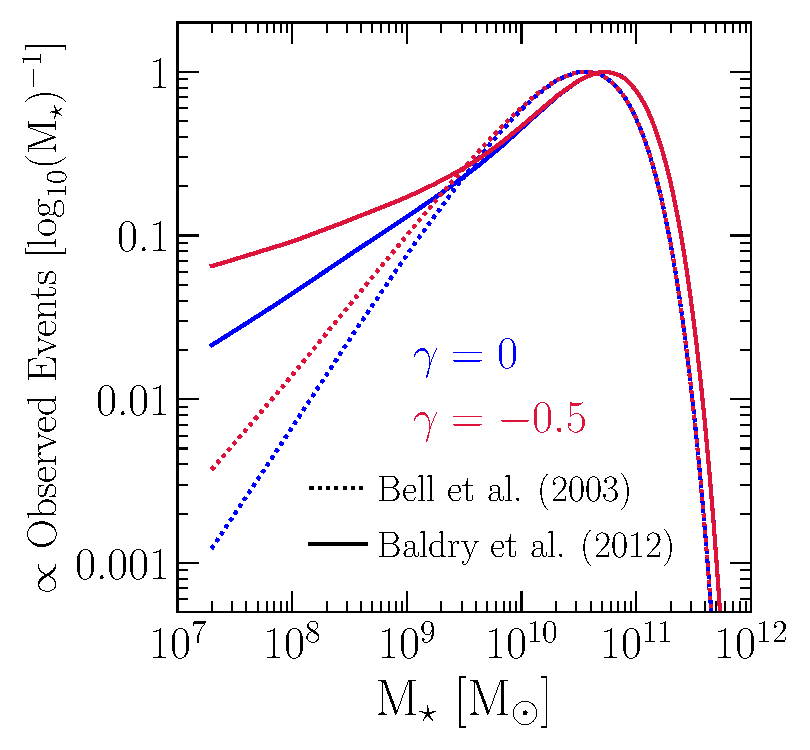
\includegraphics[scale = 0.55]{ia_massdist.pdf}
\caption{
Stellar mass distribution of SN Ia hosts.
}
\label{fig:hostmassdist}
\end{figure}

\end{itemize}

\end{document}
